\chapter{Yield Analysis}\label{sec:yield_analysis}
	\section{Introduction}
		All components on the GaAs wafer have parameter spread. That is, the performance of both the passive and active structures have an uncertainty interval.\autocite{pph25manual} The uncertainty is due to minor variations within the wafer and to larger variations between wafers. Yield analysis is performed to estimate the possible impact that these variations can cause. The analysis randomly varies parameters in the design according to their specifications (\autoref{tab:yieldparameters}). Of interest are especially gain and stability of amplifiers as well as the frequency characteristics of sensitive filters.
		
%		\begin{table}[hbt!]
%			\caption[Parameter spread intervals.]{Different components spread parameters. The values are spread uniformly.}
%			\label{tab:yieldparameters}
%			\centering
%			\begin{tabular}{ l l }
%				Component & Spread \\\hline
%				FET dV$_t$ & $\pm$\unit[0.2]{V} \\
%				Substrate height & $\pm$\unit[10]{\mum} \\
%				Spiral inductor & $\pm$5\% \\
%				Capacitor & $\pm$5.6\% \\
%				TaN Resistor & $\pm$3.6\% \\
%				GaAs Resistor & $\pm$6\% \\
%				TiWSi Resistor & $\pm$8\%
%			\end{tabular}
%		\end{table}
		\ctable[ caption = Different components' spread parameters. The values are spread uniformly. Some of the values are taken from PH25 as they aren't defined in the PPH25 manual.,
				mincapwidth = 1.0\textwidth,
				label = tab:yieldparameters,
				pos = hbt! ]
			{ l l l l }
			{\tnote[*]{An internal parameter affecting the FET's pinch-off voltage and thus the current $i_{ds}$.}}
			{	\toprule
				Component & Parameter & Spread \\\midrule
				FET transistor & $dV_t$\tmark[*] & $\pm$\unit[0.2]{V} \\
				GaAs substrate & Height & $\pm$\unit[10]{\mum} \\
				Spiral inductor & Inductance & $\pm$\unit[5]{\%} \\
				MIM capacitor & Capacitance & $\pm$\unit[5.6]{\%} \\
				TaN resistor & Resistance & $\pm$\unit[3.6]{\%} \\
				GaAs resistor & Resistance & $\pm$\unit[6]{\%} \\
				TiWSi resistor & Resistance & $\pm$\unit[8]{\%} \\\bottomrule
			}
			
		While all final results stated in the report are calculated using electromagnetic (EM) simulations, the yield calculations are performed on the electric models. This is because yield analysis with EM simulations would be too computationally intensive. However, the results from the electric models can be very far from the EM results. The yield analysis should therefore be regarded as a measure of how the result can vary due to process spread and not as the actual result.


	\section{Amplifier LO}\label{yieldlo}
		Yield analysis of amplifier LO is shown in \autoref{tab:lo_spread}, \autoref{fig:lo_spread}.


		\begin{table}[hbt!]
			\caption[Amplifier LO performance with spread.]{Amplifier LO typical performance with spread at $P_{LO}=\unit[-2]{dBm}$.}
			\label{tab:lo_spread}
			\centering
			\begin{tabular}{ l l } \toprule
				Parameter & Performance \\\midrule
				Delivered Power & $\unit[5\pm2]{dB}$ \\
				Return Loss Input & $\unit[15\pm2 ]{dB}$ \\
				Stability & $K>1$ \\
				%$P_{1dB}$ (Input) & $\unit[\pm ]{dBm}$ \\
				Power Consumption &  $\unit[100\pm 5]{mW}$ \\\bottomrule
			\end{tabular}
		\end{table}		
		

		\begin{figure}[hp!]
			\centering 
			\subfloat[][Delivered power at input power -2 dBm.]{
				\includerect{0.5\textwidth}{fig/amplifiers/lo/lo_delivered_power_spread_-2dBm}
				\label{fig:lo_delivered_power_spread_-2dBm}
			}
			\subfloat[][Delivered power at input power -4 dBm.]{
				\includerect{0.5\textwidth}{fig/amplifiers/lo/lo_delivered_power_spread_-4dBm}
				\label{fig:lo_delivered_power_spread_-4dBm}
			}			
			\\
			\subfloat[][Input reflection coefficient $S_{11}$ at input power -2 dBm. Active frequency range is 5.04 to 5.54 GHz]{
				\includerect{0.5\textwidth}{fig/amplifiers/lo/lo_reflections_spread}
				\label{fig:lo_reflections_spread}
			}
			\subfloat[][Input reflection coefficient $S_{11}$ at input power -4 dBm. Active frequency range is 5.04 to 5.54 GHz]{
				\includerect{0.5\textwidth}{fig/amplifiers/lo/lo_reflections_spread_-4dBm}
				\label{fig:lo_reflections_spread}
			} \\	
			\subfloat[][Stability measure K. Note that even though the electric model has $K<1$ at 70 GHz the EM model is stable.]{
				\includerect{0.5\textwidth}{fig/amplifiers/lo/lo_stability_spread}
				\label{fig:lo_stability_spread}
			} 
			\subfloat[][Power consumption at input power -2 dBm.]{
				\includerect{0.5\textwidth}{fig/amplifiers/lo/lo_power_consumption_spread}
				\label{fig:lo_power_consumption_spread}
			}
			\caption[Yield analysis of amplifier LO.]{Yield analysis of amplifier LO at input power \unit[-2 and -4]{dBm}. The spread analyzed with the electric circuit model gives a hint of the spread for the more accurate electromagnetic simulation.}\label{fig:lo_spread}
		\end{figure}
		

	\section{Amplifier IF1}\label{sec:yieldif1}
		Yield analysis of amplifier IF1 is shown in \autoref{tab:yieldif1} and \autoref{fig:yieldif1}.
		
		\begin{table}[hbt!]
			\caption[Amplifier IF1 performance with spread.]{Amplifier IF1 typical performance with spread.}
			\label{tab:yieldif1}
			\centering
			\begin{tabular}{ l l } \toprule
				Parameter & Performance \\\midrule
				Gain & $\unit[11.5\pm 0.75]{dB}$ \\
				Return Loss Input & $\unit[14.4\pm 5]{dB}$ \\
				Return Loss Output & $\unit[16.9\pm 1.5]{dB}$ \\
				Stability & $K>1$ \\
				$P_{1dB}$ (Input) & $\unit[6.2\pm 1]{dBm}$ \\
				Power Consumption &  $\unit[290\pm 40]{mW}$ \\\bottomrule
			\end{tabular}
		\end{table}
		
		\begin{figure}[hp!]
			\centering 
			\subfloat[][Gain.]{
				\includerect{0.5\textwidth}{fig/yield/s21if1}
				\label{fig:yieldif1gain}
			}
			\subfloat[][Input reflection coefficient S11.]{
				\includerect{0.5\textwidth}{fig/yield/s11if1}
				\label{fig:yieldif1s11}
			} \\
			\subfloat[][Output reflection coefficient S22.]{
				\includerect{0.5\textwidth}{fig/yield/s22if1}
				\label{fig:yieldif1s22}
			}
			\subfloat[][Stability measure K. Note that even though the electric model has $K<1$ at 60 GHz the EM model is stable.]{
				\includerect{0.5\textwidth}{fig/yield/stabkif1}
				\label{fig:yieldif1stability}
			} \\
			\subfloat[][Power compression.]{
				\includerect{0.5\textwidth}{fig/yield/compressif1}
				\label{fig:yieldif1compress}
			}
			\subfloat[][Power consumption.]{
				\includerect{0.5\textwidth}{fig/yield/powerif1}
				\label{fig:yieldif1power}
			}
			\caption[Yield analysis of amplifier IF1.]{Yield analysis of amplifier IF1. The spread analyzed with the electric circuit model gives a hint of the spread for the more accurate electromagnetic simulation.}\label{fig:yieldif1}
		\end{figure}
				
%		\begin{figure}[hbt!]
%			\centering
%			%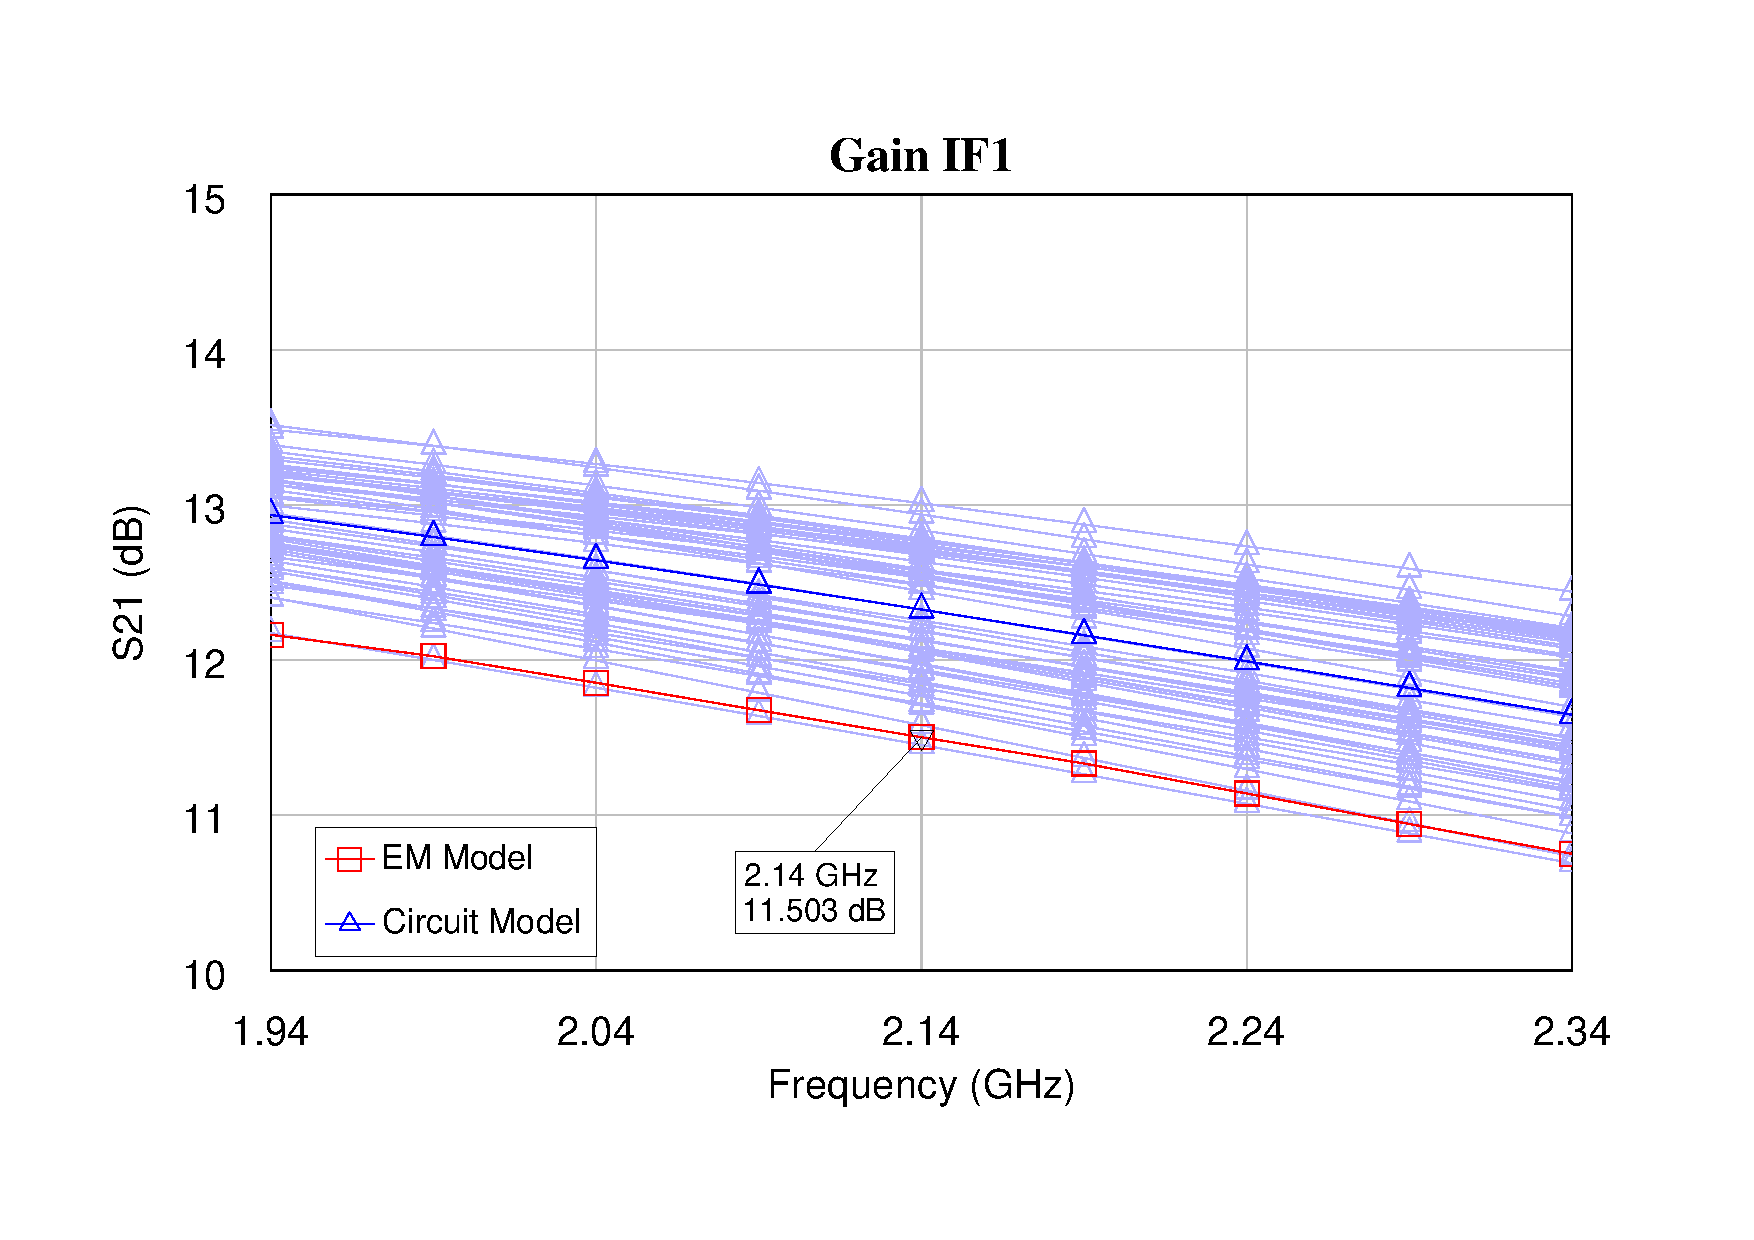
\includegraphics[width=0.9\textwidth,trim=45 60 70 60]{fig/yield/s21if1}
%			\includerect{1.0\textwidth}{fig/yield/s21if1}
%			\caption[Yield analysis of gain for amplifier IF1.]{Gain of amplifier IF 1. The spread analyzed with the electric circuit model gives a hint of the spread for the more accurate electromagnetic simulation.}\label{fig:yieldif1gain}
%		\end{figure}
%		
%		\begin{figure}[hbt!]
%			\centering
%			%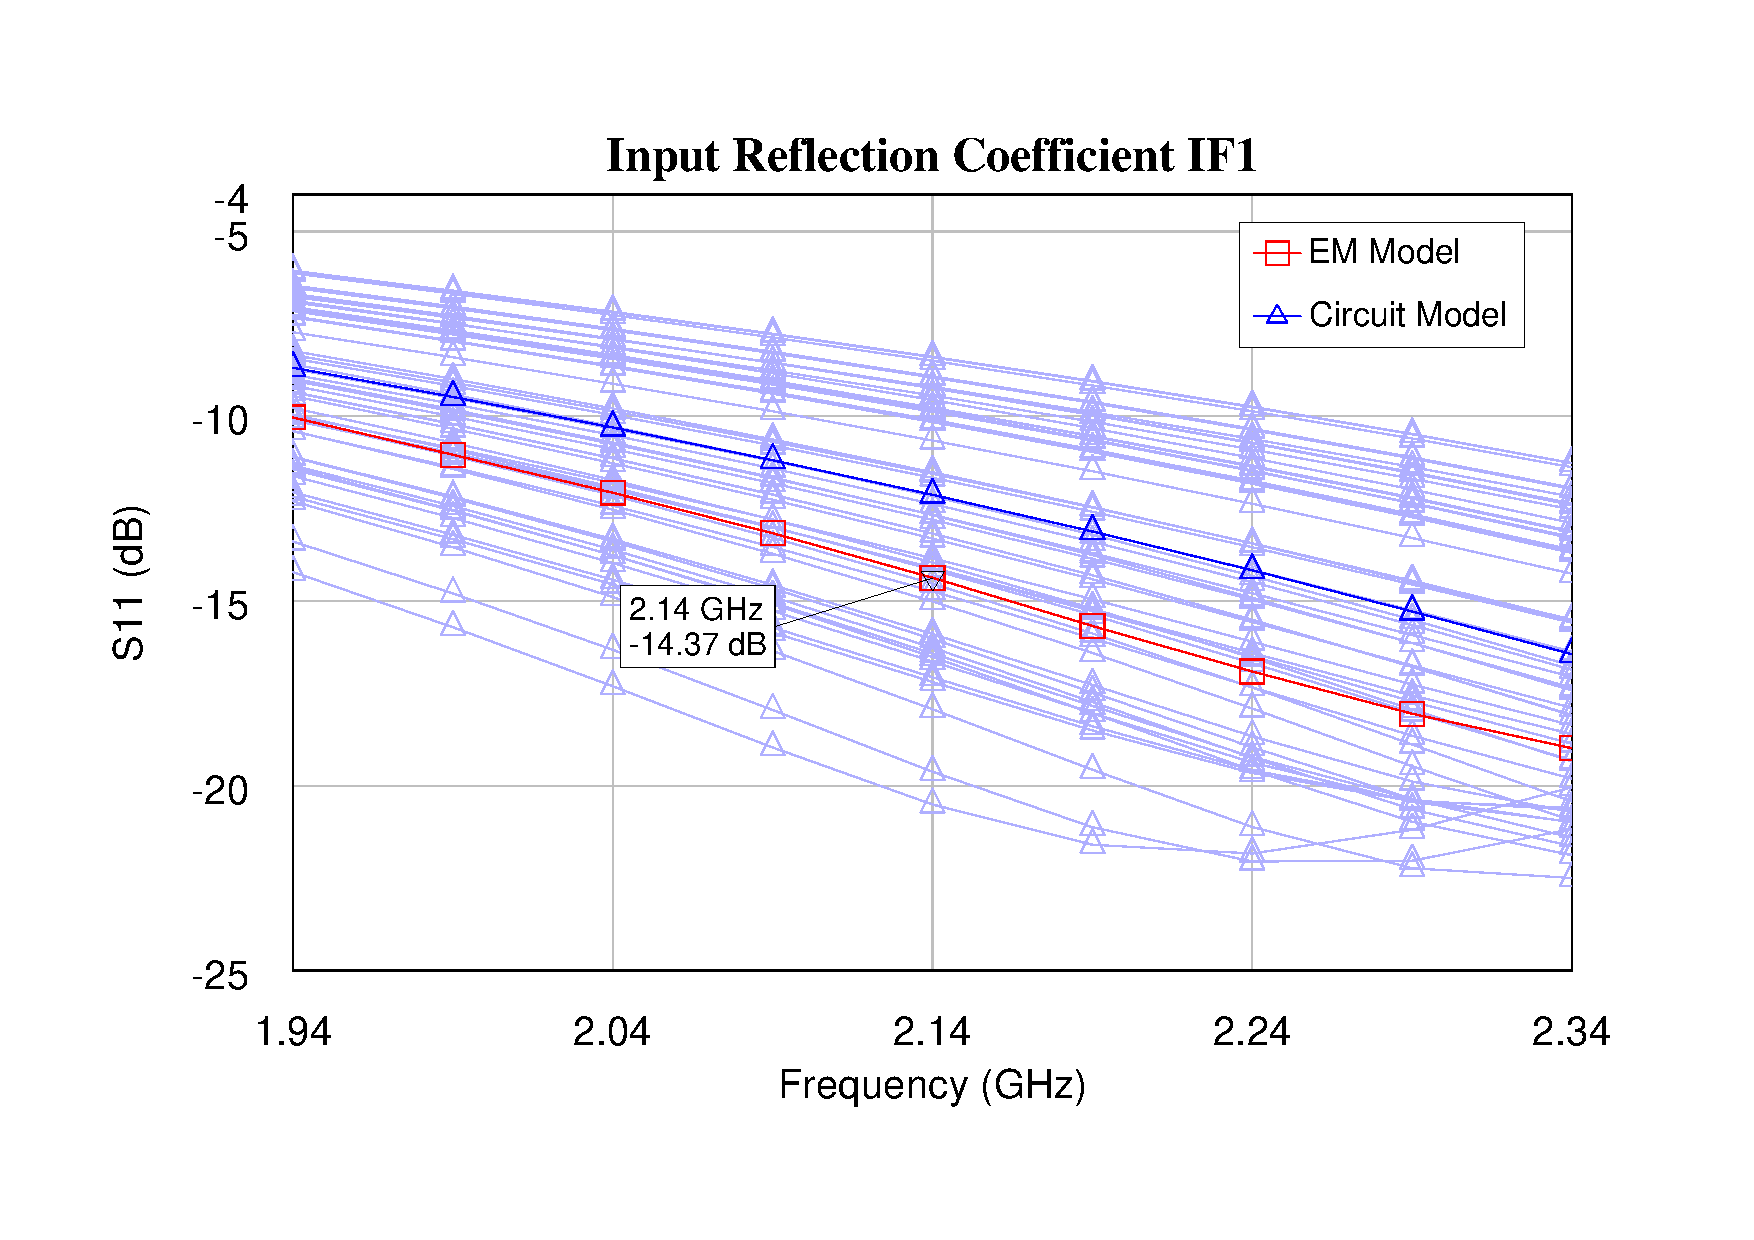
\includegraphics[width=0.9\textwidth,trim=60 70 80 90]{fig/yield/s11if1}
%			\includerect{1.0\textwidth}{fig/yield/s11if1}
%			\caption[Yield analysis of S11 for amplifier IF1.]{Input reflection coefficient S11 of amplifier IF 1. The spread analyzed with the electric circuit model gives a hint of the spread for the more accurate electromagnetic simulation.}\label{fig:yieldif1s11}
%		\end{figure}
%		
%		\begin{figure}[hbt!]
%			\centering
%			%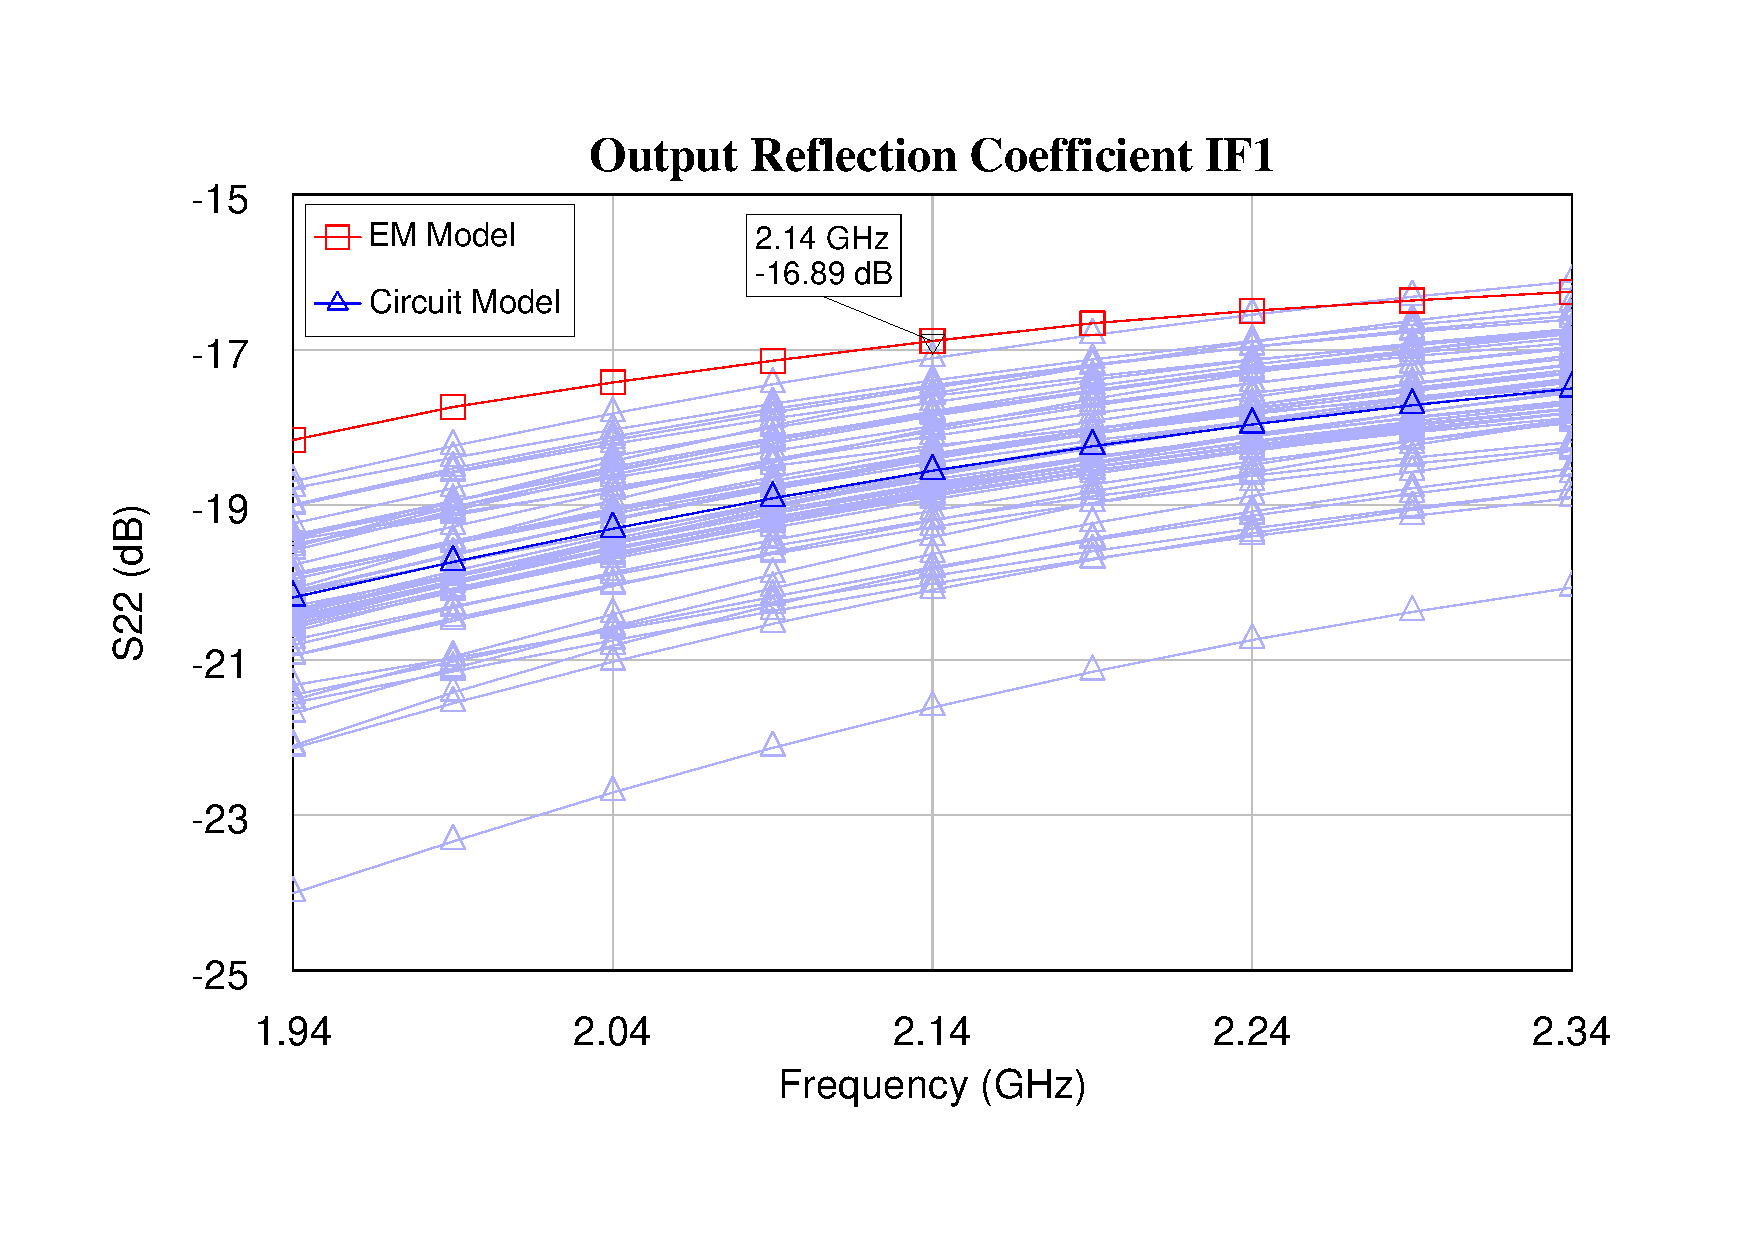
\includegraphics[width=0.9\textwidth]{fig/yield/s22if1}
%			\includerect{1.0\textwidth}{fig/yield/s22if1}
%			\caption[Yield analysis of S22 for amplifier IF1.]{Output reflection coefficient S22 of amplifier IF 1. The spread analyzed with the electric circuit model gives a hint of the spread for the more accurate electromagnetic simulation.}\label{fig:yieldif1s22}
%		\end{figure}
%				
%		\begin{figure}[hbt!]
%			\centering
%			%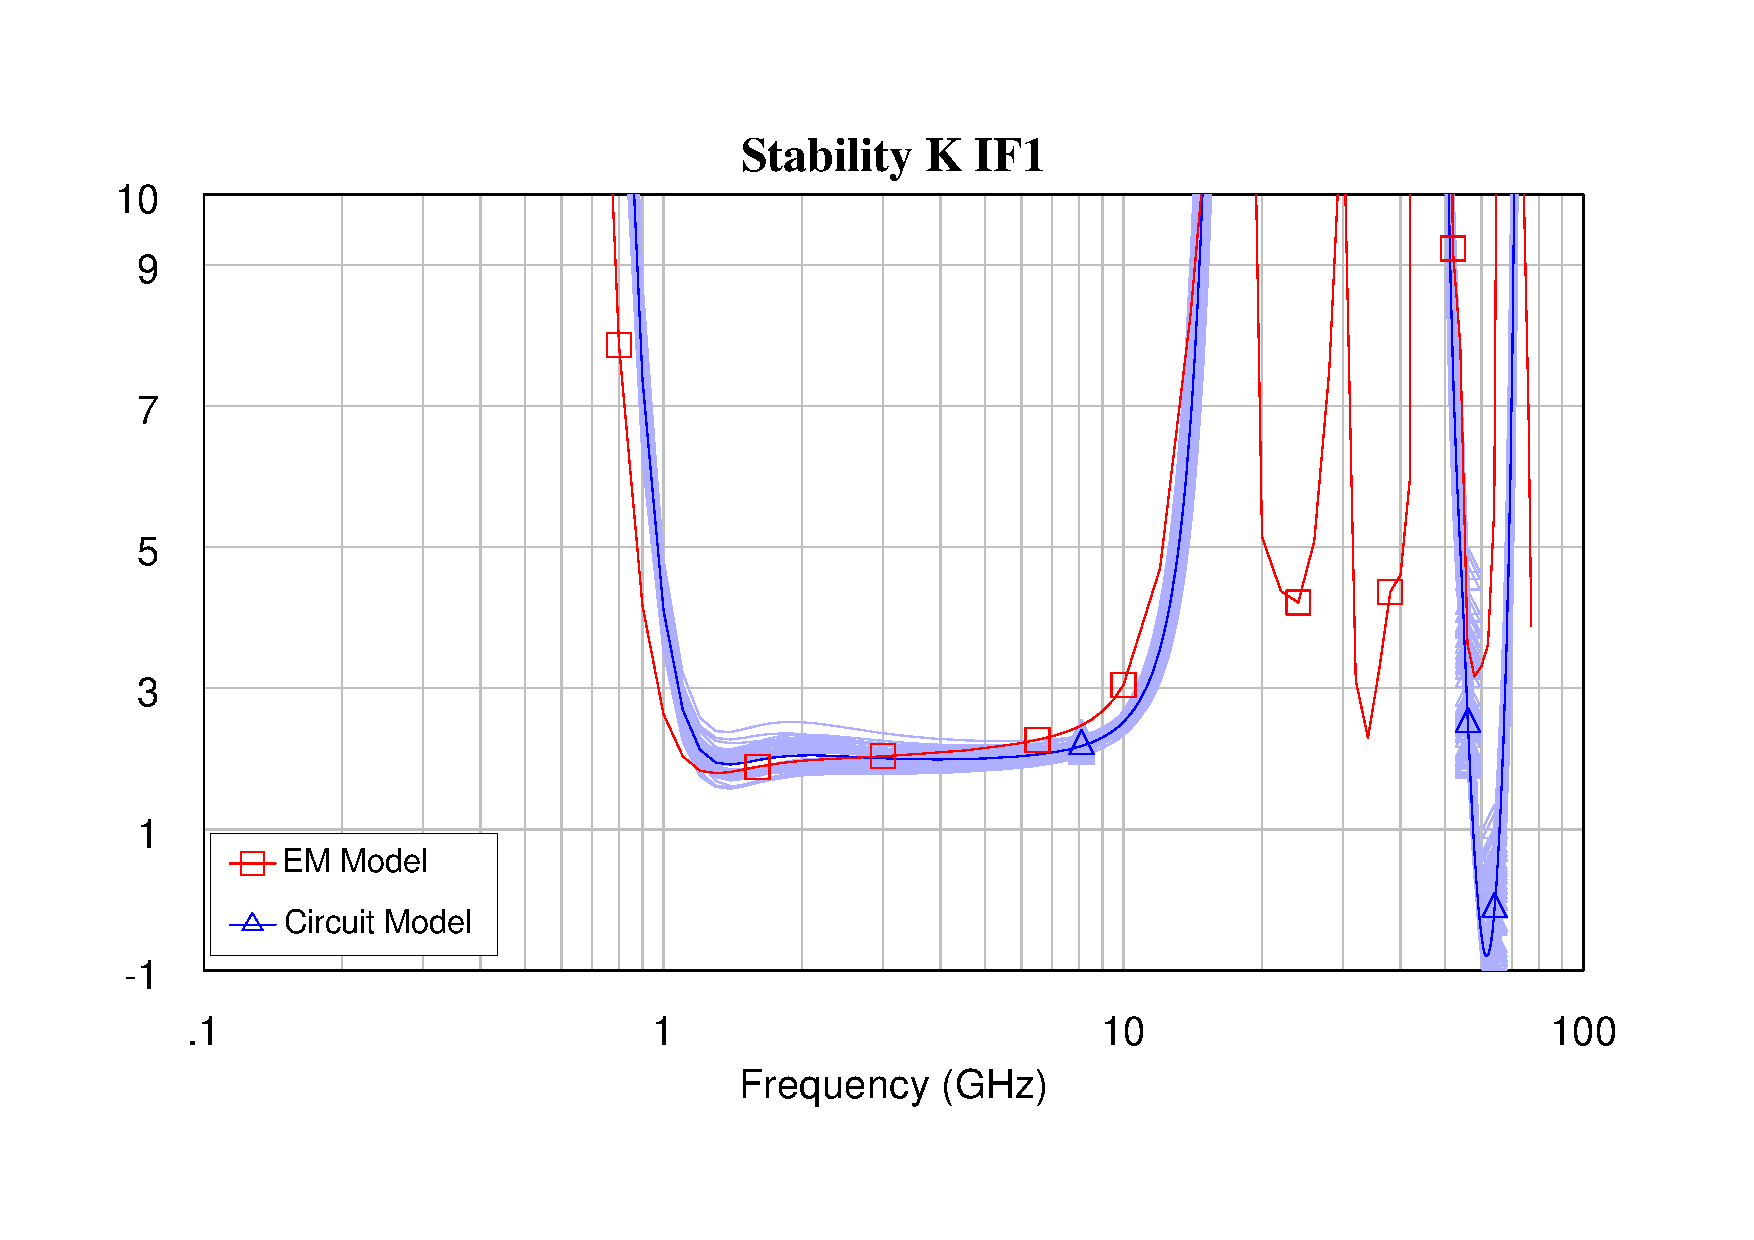
\includegraphics[width=0.9\textwidth]{fig/yield/stabkif1}
%			\includerect{1.0\textwidth}{fig/yield/stabkif1}
%			\caption[Yield analysis of stability for amplifier IF1.]{Stability measure K for amplifier IF 1. The spread analyzed with the electric circuit model gives a hint of the spread for the more accurate electromagnetic simulation. Note that even though the electric model has $K<1$ at \unit[60]{GHz} the EM model is stable.}\label{fig:yieldif1stability}
%		\end{figure}
%		
%		\begin{figure}[hbt!]
%			\centering
%			%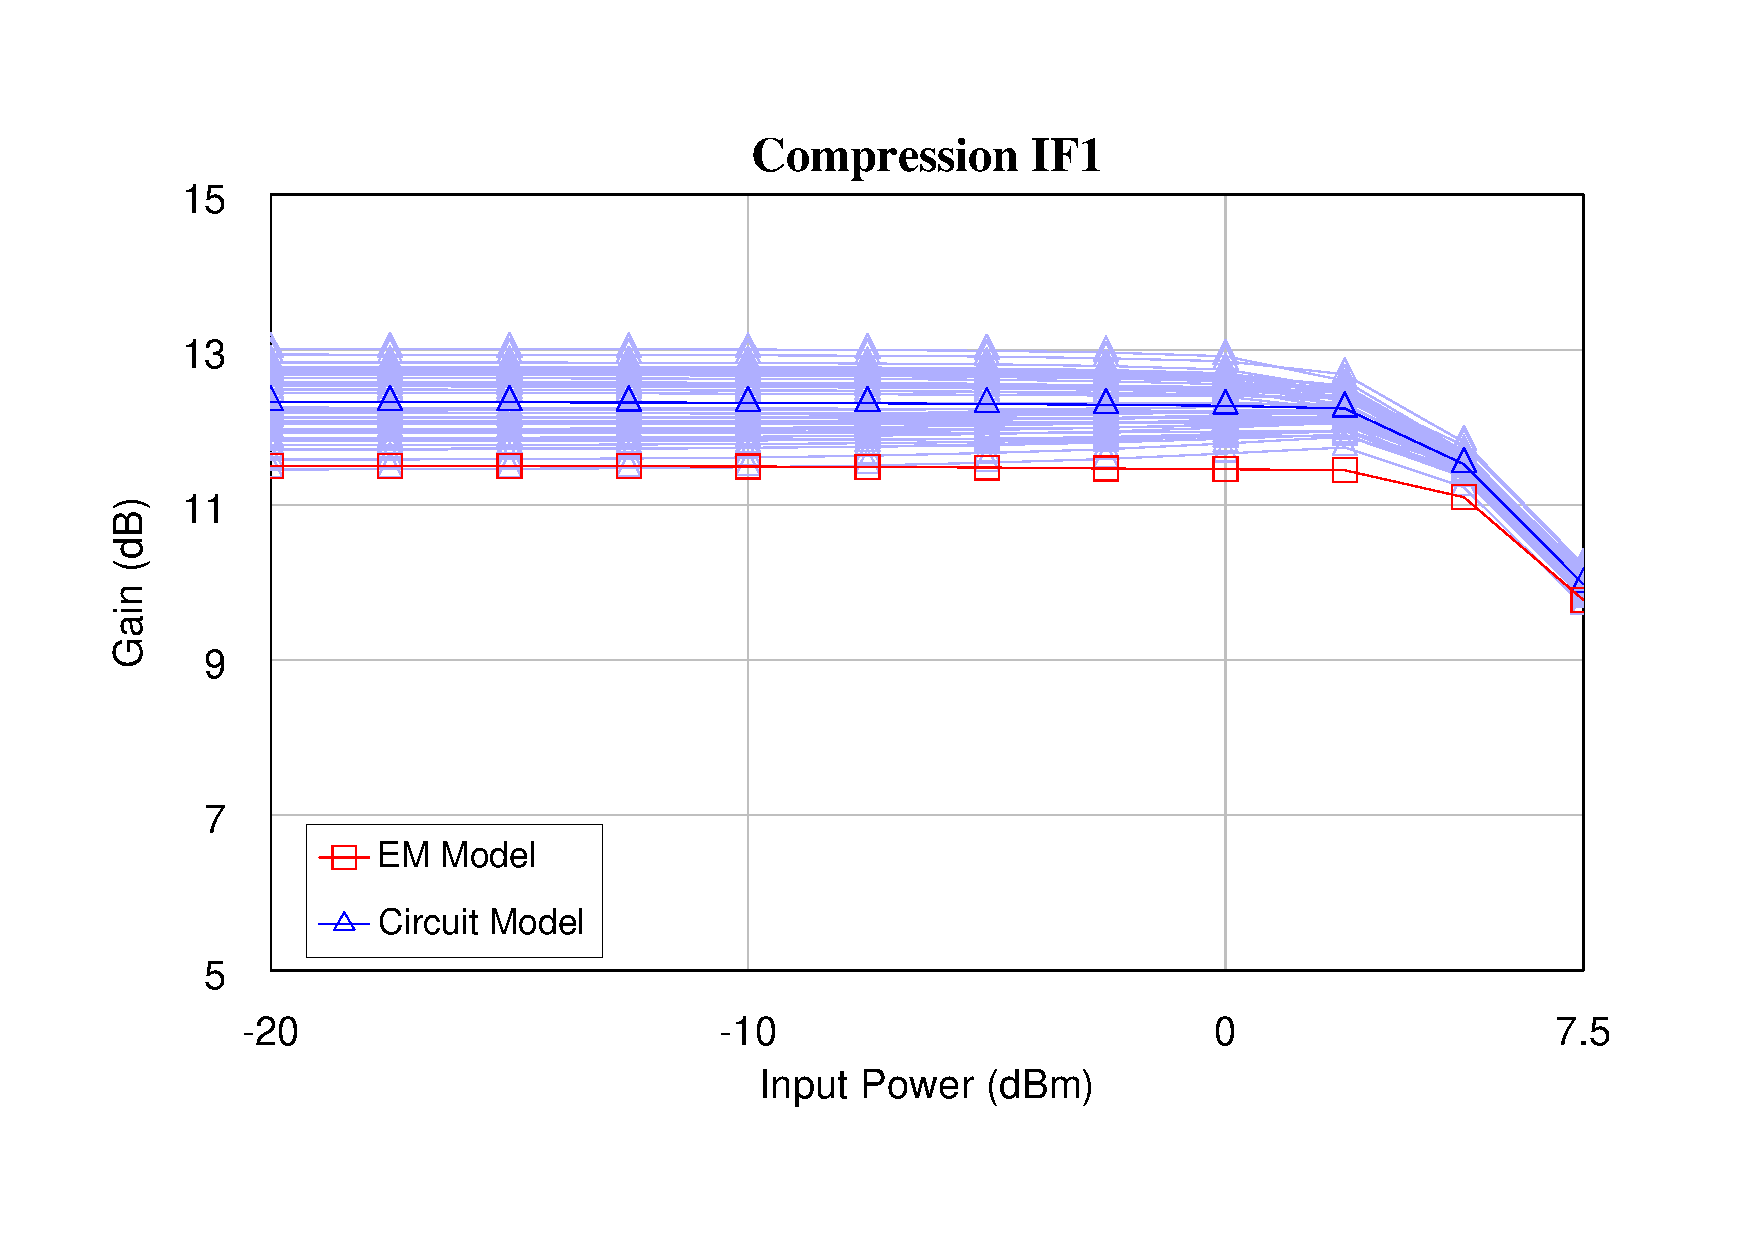
\includegraphics[width=0.9\textwidth]{fig/yield/compressif1}
%			\includerect{1.0\textwidth}{fig/yield/compressif1}
%			\caption[Yield analysis of the power compression for amplifier IF1.]{Power compression of amplifier IF 1 at \unit[2.14]{GHz}. The spread analyzed with the electric circuit model gives a hint of the spread for the more accurate electromagnetic simulation.}\label{fig:yieldif1compress}
%		\end{figure}
%		
%		\begin{figure}[hbt!]
%			\centering
%			%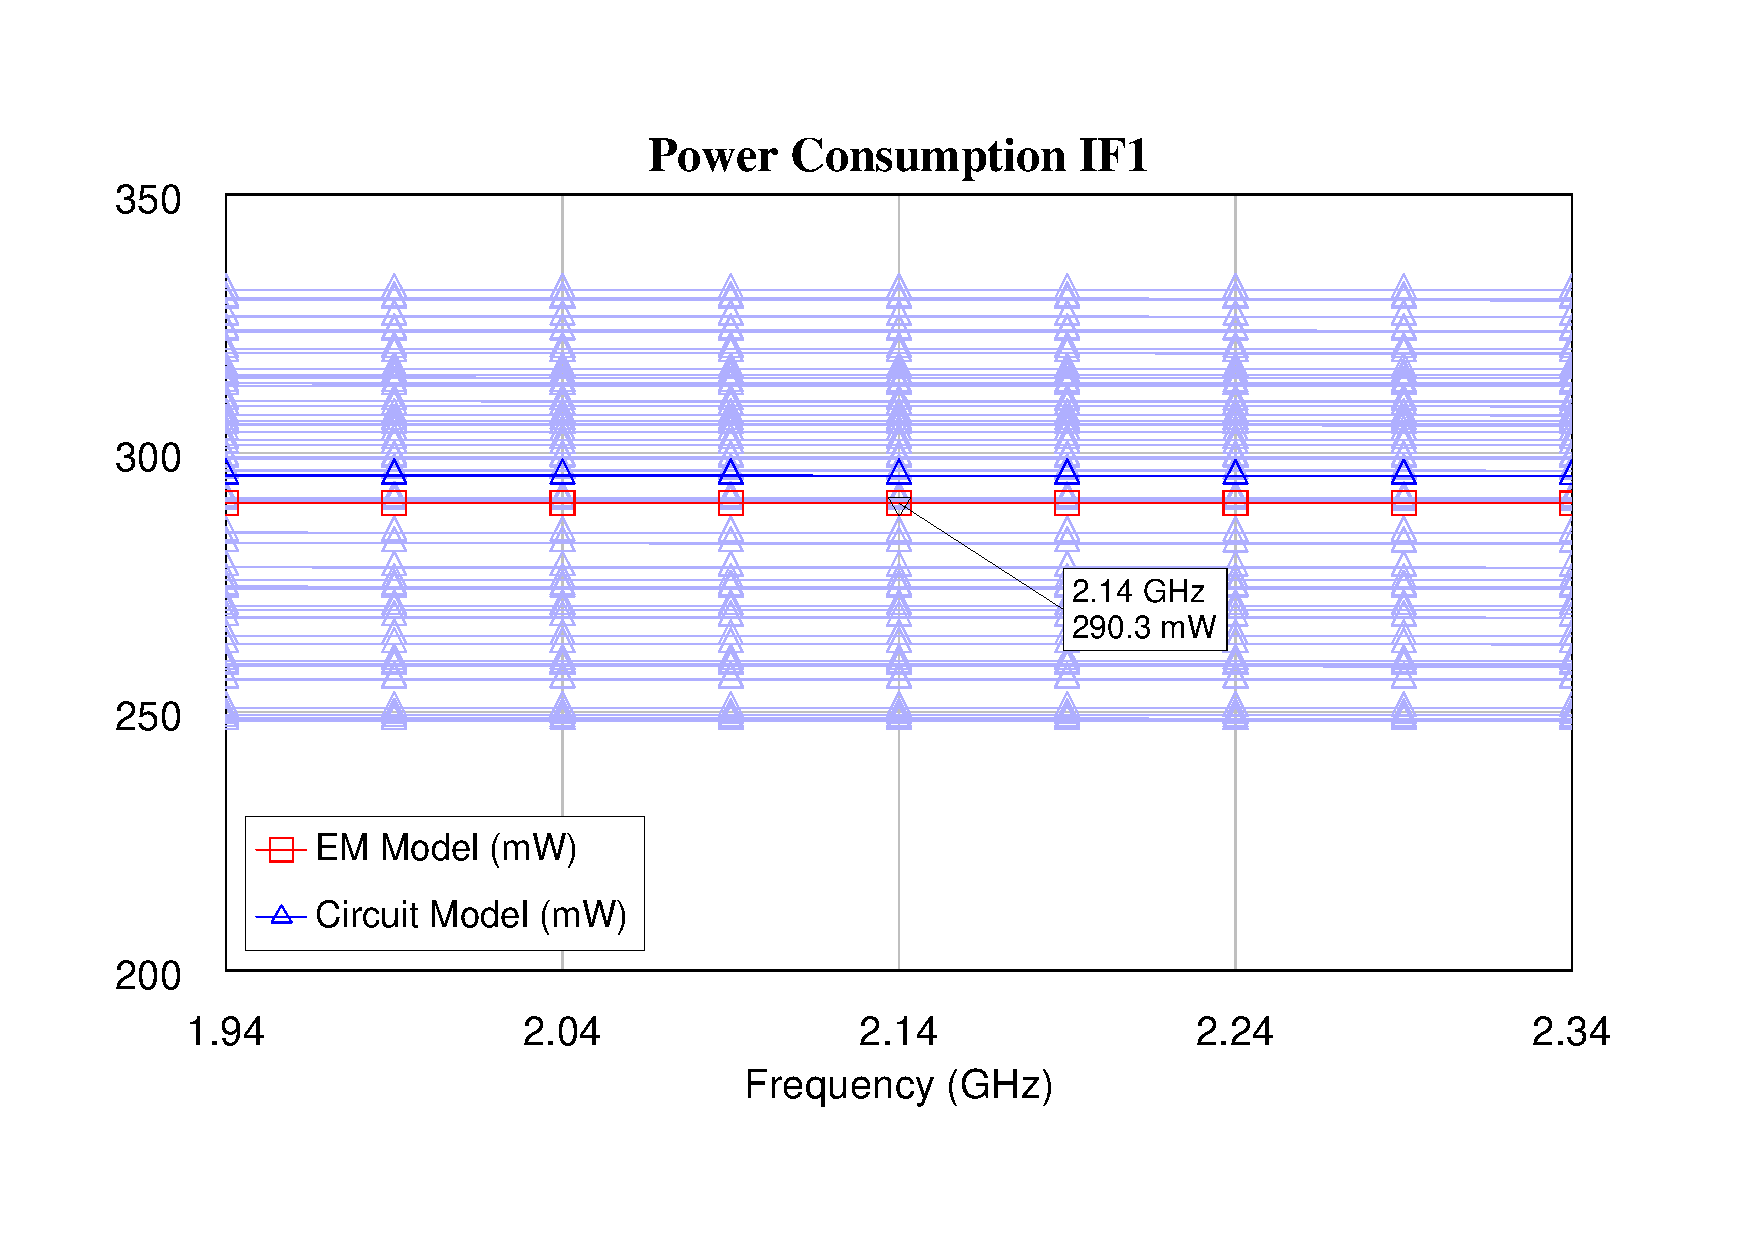
\includegraphics[width=0.9\textwidth]{fig/yield/powerif1}
%			\includerect{1.0\textwidth}{fig/yield/powerif1}
%			\caption[Yield analysis of power consumption for amplifier IF1.]{Power consumption of amplifier IF 1. The spread analyzed with the electric circuit model gives a hint of the spread for the more accurate electromagnetic simulation.}\label{fig:yieldif1power}
%		\end{figure}

	\section{Amplifier IF2}\label{sec:yieldif2}
		Yield analysis of amplifier IF2 is shown in \autoref{tab:yieldif2} and \autoref{fig:yieldif2}.
		
		\begin{table}[hbt!]
			\caption[Amplifier IF2 performance with spread.]{Amplifier IF2 typical performance with spread.}
			\label{tab:yieldif2}
			\centering
			\begin{tabular}{ l l } \toprule
				Parameter & Performance \\\midrule
				Gain & $\unit[12.1\pm 0.5]{dB}$ \\
				Return Loss Input & $\unit[25.5\pm 6]{dB}$ \\
				Return Loss Output & $\unit[19.7\pm 3]{dB}$ \\
				Stability & $K>1$ \\
				$P_{1dB}$ (Input) & $\unit[10.4\pm 1]{dBm}$ \\
				Power Consumption &  $\unit[550\pm 70]{mW}$ \\\bottomrule
			\end{tabular}
		\end{table}
		
		\begin{figure}[hp!]
			\centering 
			\subfloat[][Gain.]{
				\includerect{0.5\textwidth}{fig/yield/s21if2}
				\label{fig:yieldif2gain}
			}
			\subfloat[][Input reflection coefficient S11.]{
				\includerect{0.5\textwidth}{fig/yield/s11if2}
				\label{fig:yieldif2s11}
			} \\
			\subfloat[][Output reflection coefficient S22.]{
				\includerect{0.5\textwidth}{fig/yield/s22if2}
				\label{fig:yieldif2s22}
			}
			\subfloat[][Stability measure K.]{
				\includerect{0.5\textwidth}{fig/yield/stabkif2}
				\label{fig:yieldif2stability}
			} \\
			\subfloat[][Power compression.]{
				\includerect{0.5\textwidth}{fig/yield/compressif2}
				\label{fig:yieldif2compress}
			}
			\subfloat[][Power consumption.]{
				\includerect{0.5\textwidth}{fig/yield/powerif2}
				\label{fig:yieldif2power}
			}
			\caption[Yield analysis of amplifier IF2.]{Yield analysis of amplifier IF2. The spread analysed with the electric circuit model gives a hint of the spread for the more accurate electromagnetic simulation.}\label{fig:yieldif2}
		\end{figure}
		
%		\begin{figure}[hbt!]
%			\centering
%			%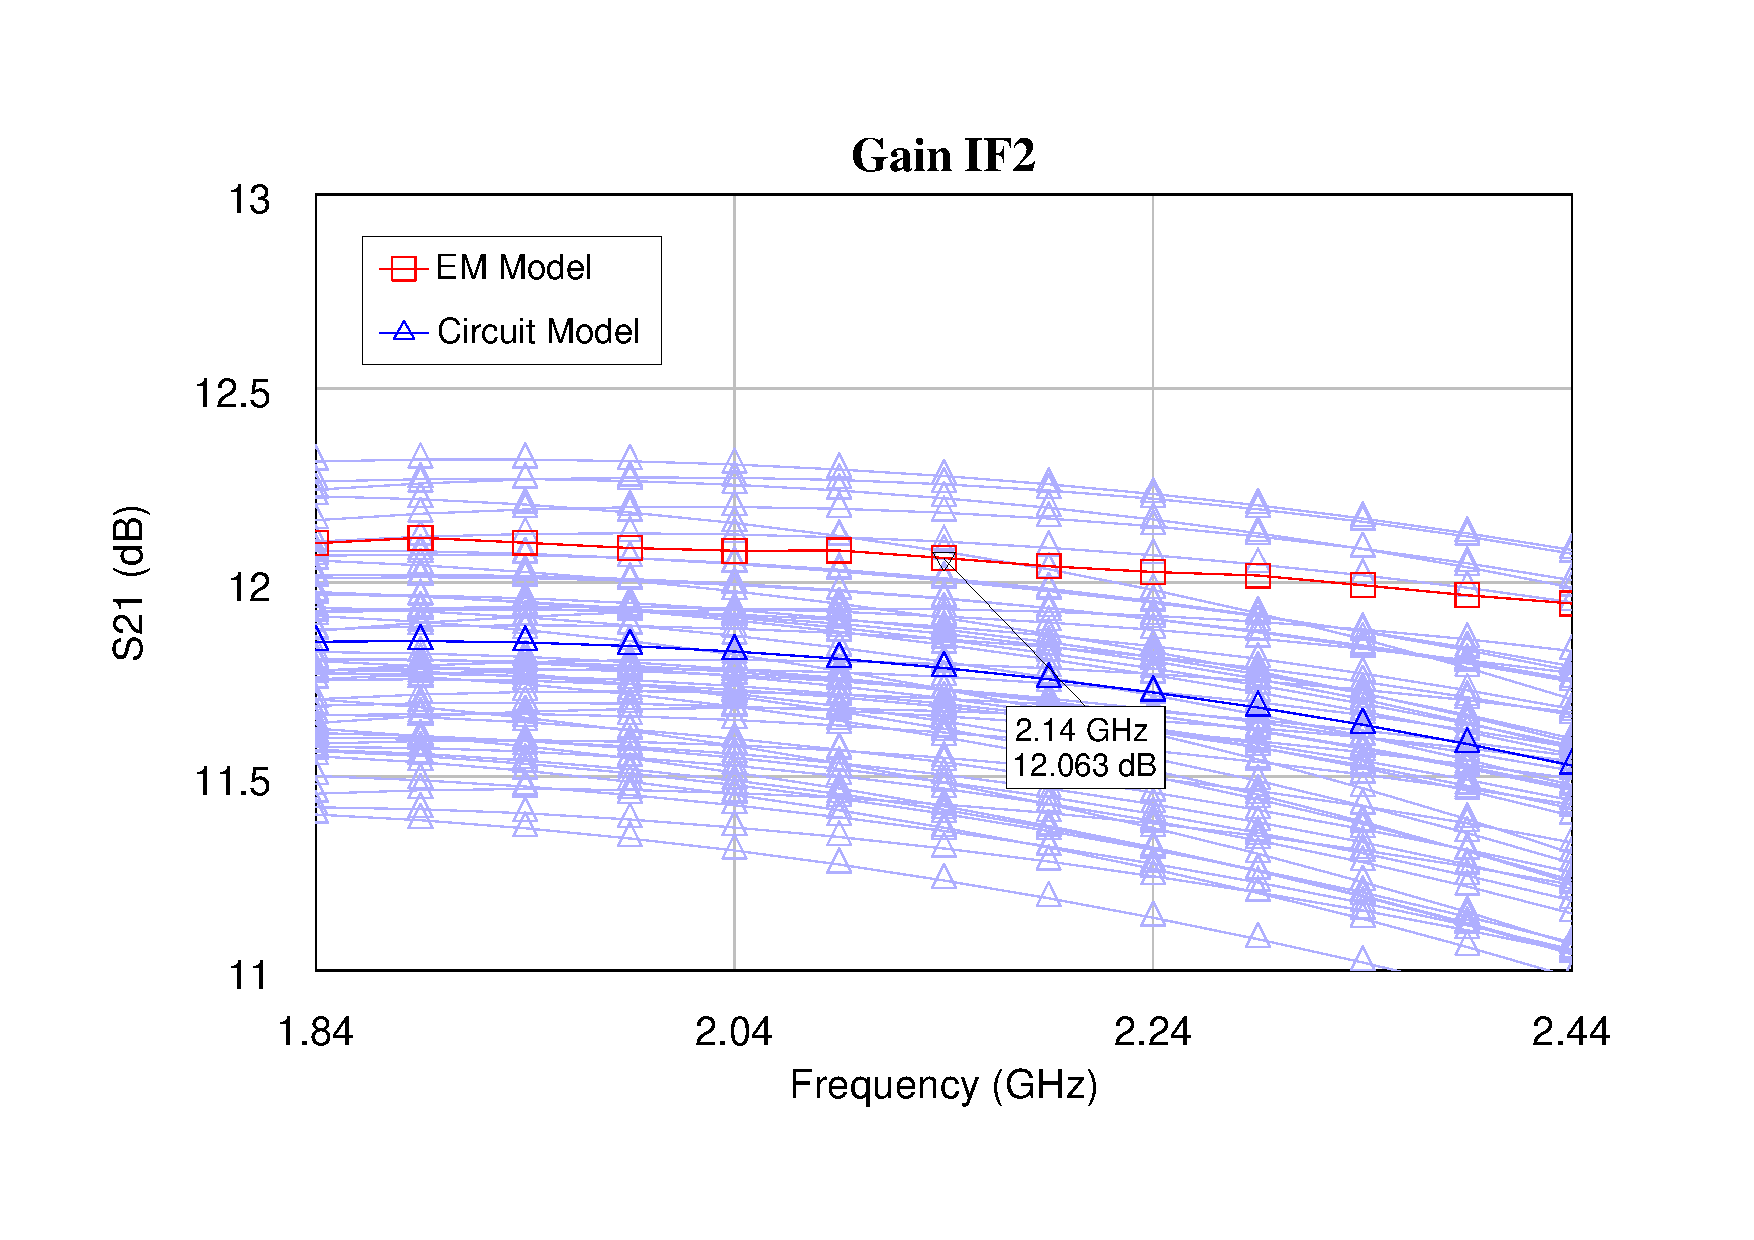
\includegraphics[width=0.9\textwidth]{fig/yield/s21if2}
%			\includerect{1.0\textwidth}{fig/yield/s21if2}
%			\caption[Yield analysis of gain for amplifier IF2.]{Gain of amplifier IF 2. The spread analysed with the electric circuit model gives a hint of the spread for the more accurate electromagnetic simulation.}\label{fig:yieldif2gain}
%		\end{figure}
%		
%		\begin{figure}[hbt!]
%			\centering
%			%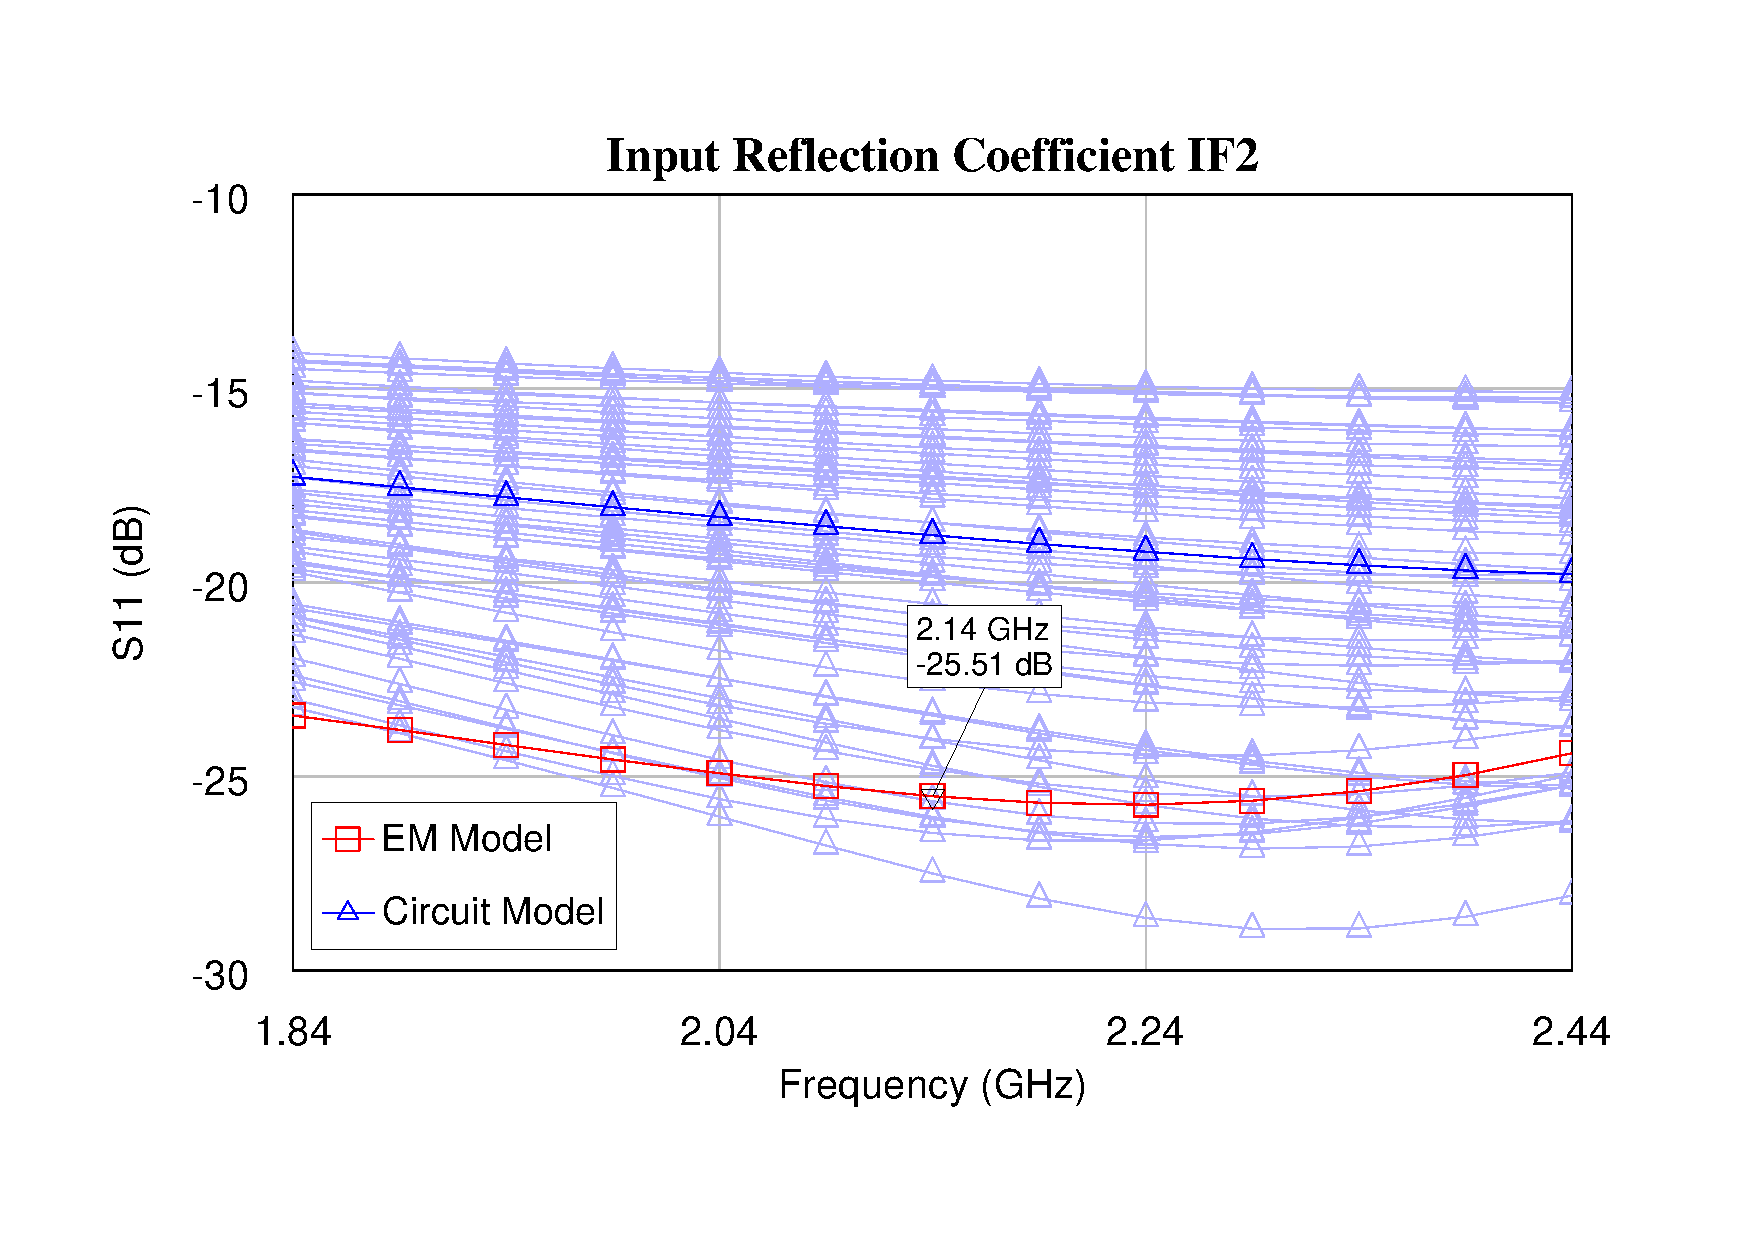
\includegraphics[width=0.9\textwidth]{fig/yield/s11if2}
%			\includerect{1.0\textwidth}{fig/yield/s11if2}
%			\caption[Yield analysis of S11 for amplifier IF2.]{Input reflection coefficient S11 of amplifier IF 2. The spread analysed with the electric circuit model gives a hint of the spread for the more accurate electromagnetic simulation.}\label{fig:yieldif2s11}
%		\end{figure}
%		
%		\begin{figure}[hbt!]
%			\centering
%			%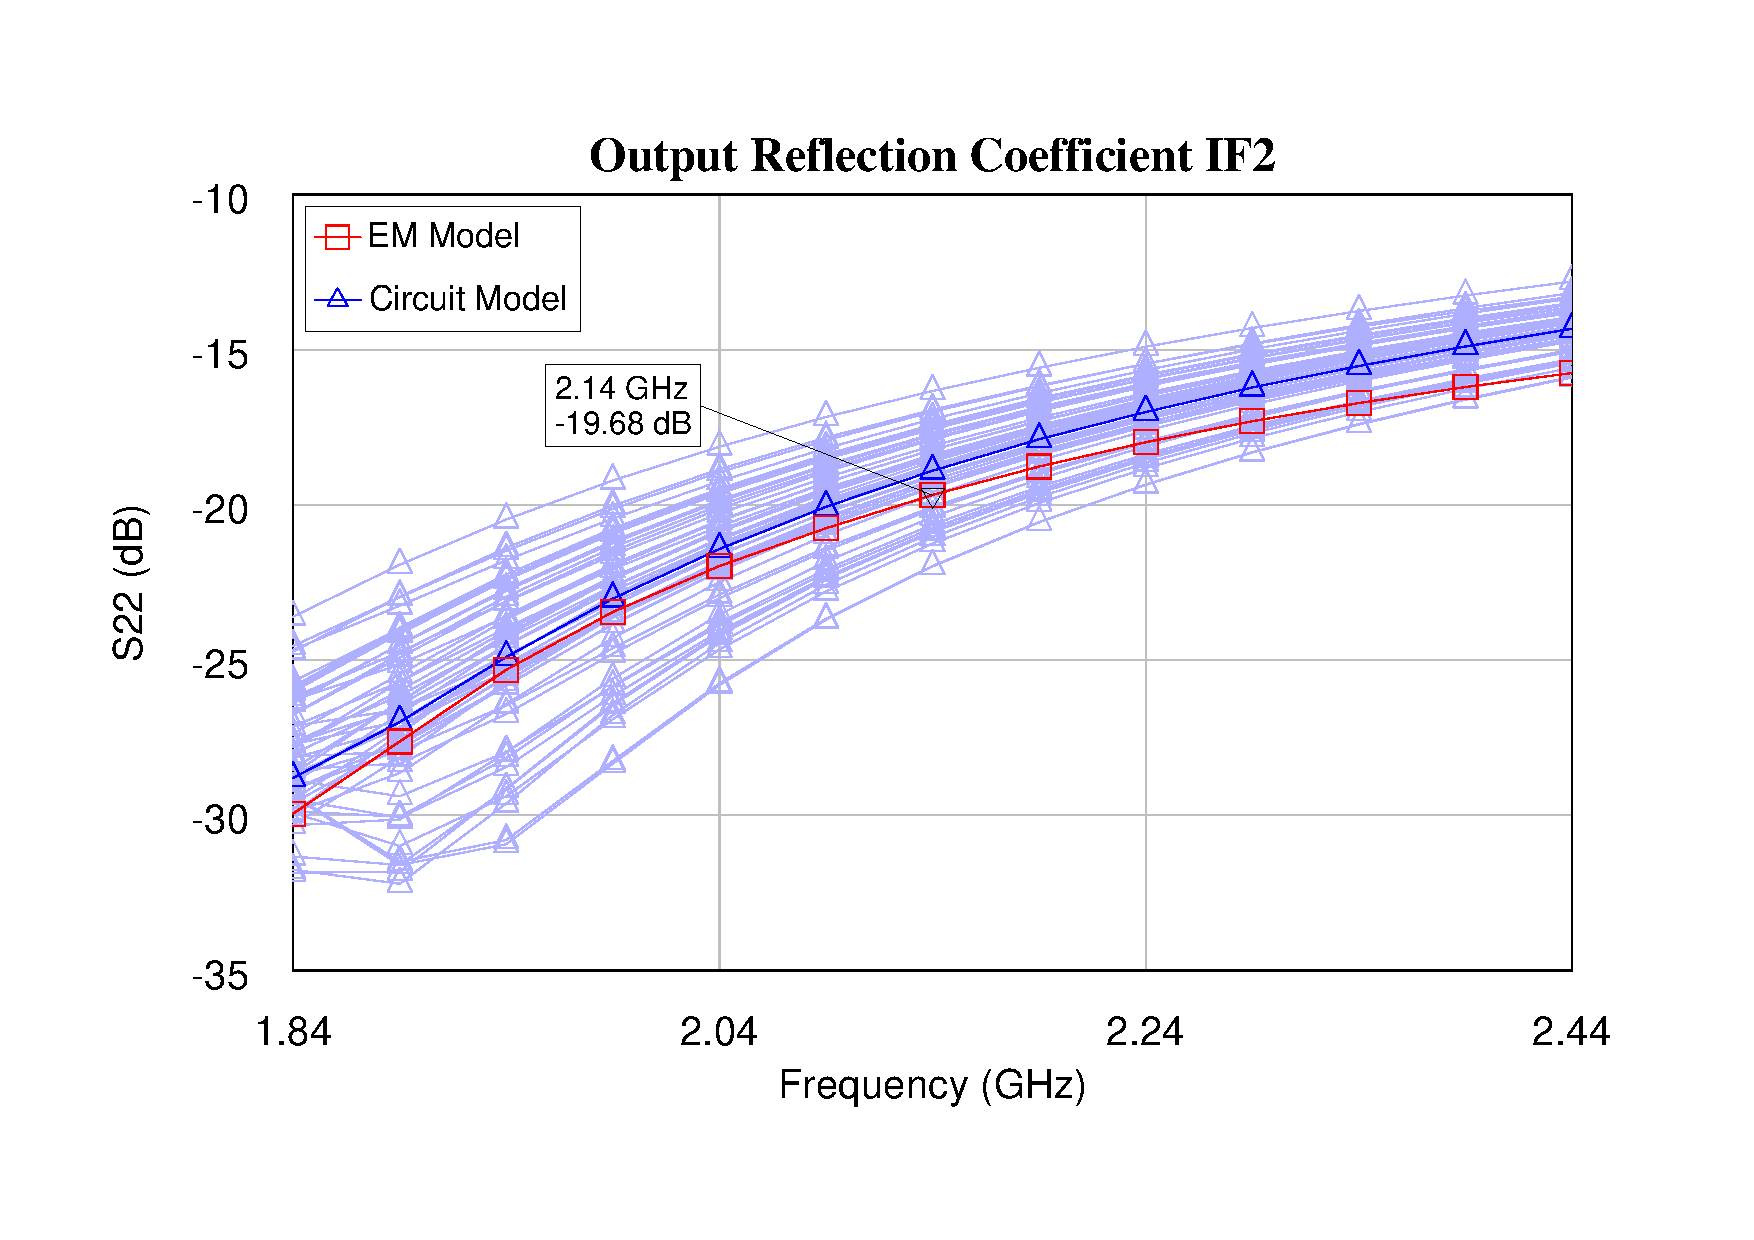
\includegraphics[width=0.9\textwidth]{fig/yield/s22if2}
%			\includerect{1.0\textwidth}{fig/yield/s22if2}
%			\caption[Yield analysis of S22 for amplifier IF2.]{Output reflection coefficient S22 of amplifier IF 2. The spread analysed with the electric circuit model gives a hint of the spread for the more accurate electromagnetic simulation.}\label{fig:yieldif2s22}
%		\end{figure}
%				
%		\begin{figure}[hbt!]
%			\centering
%			%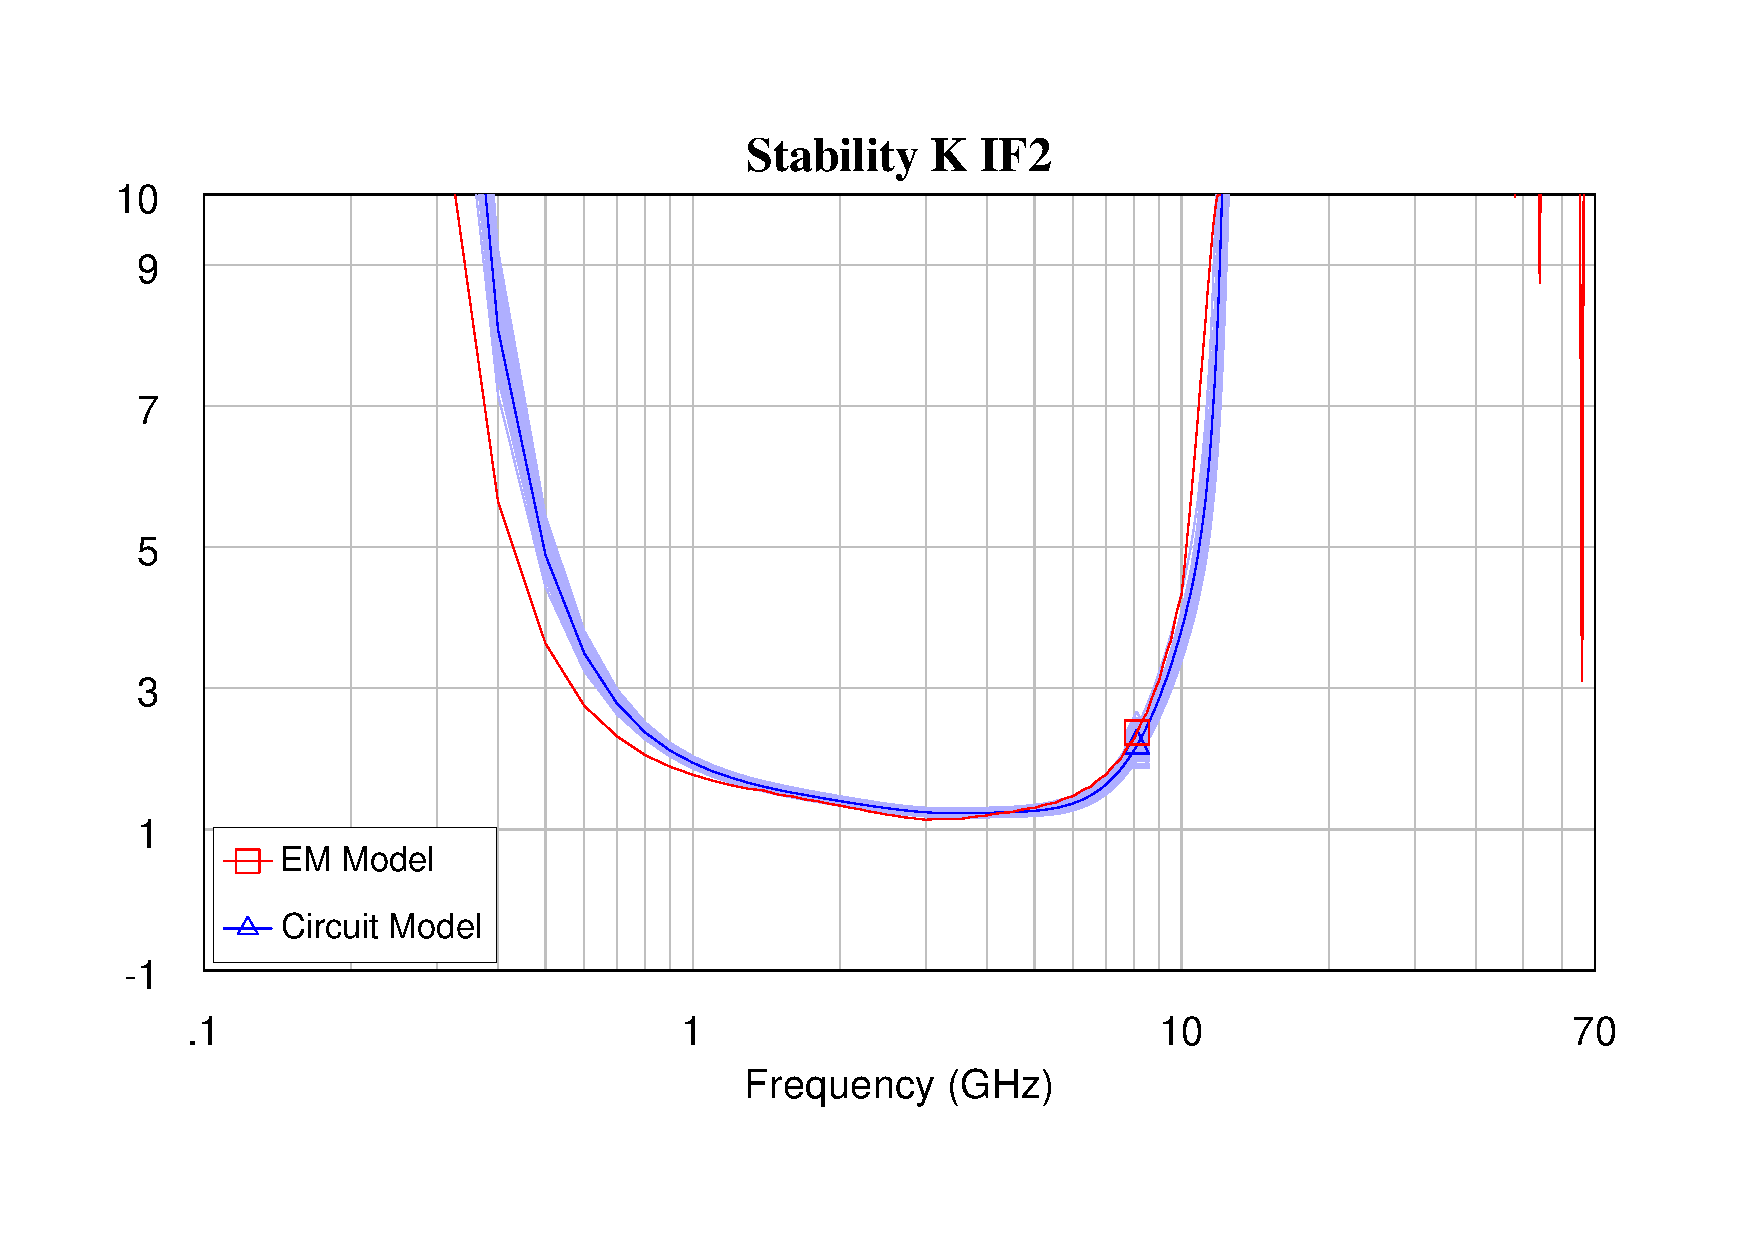
\includegraphics[width=0.9\textwidth]{fig/yield/stabkif2}
%			\includerect{1.0\textwidth}{fig/yield/stabkif2}
%			\caption[Yield analysis of stability for amplifier IF2.]{Stability measure K for amplifier IF 2. The spread analysed with the electric circuit model gives a hint of the spread for the more accurate electromagnetic simulation. Note that even though the electric model has $K<1$ at \unit[60]{GHz} the EM model is stable.}\label{fig:yieldif2stability}
%		\end{figure}
%		
%		\begin{figure}[hbt!]
%			\centering
%			%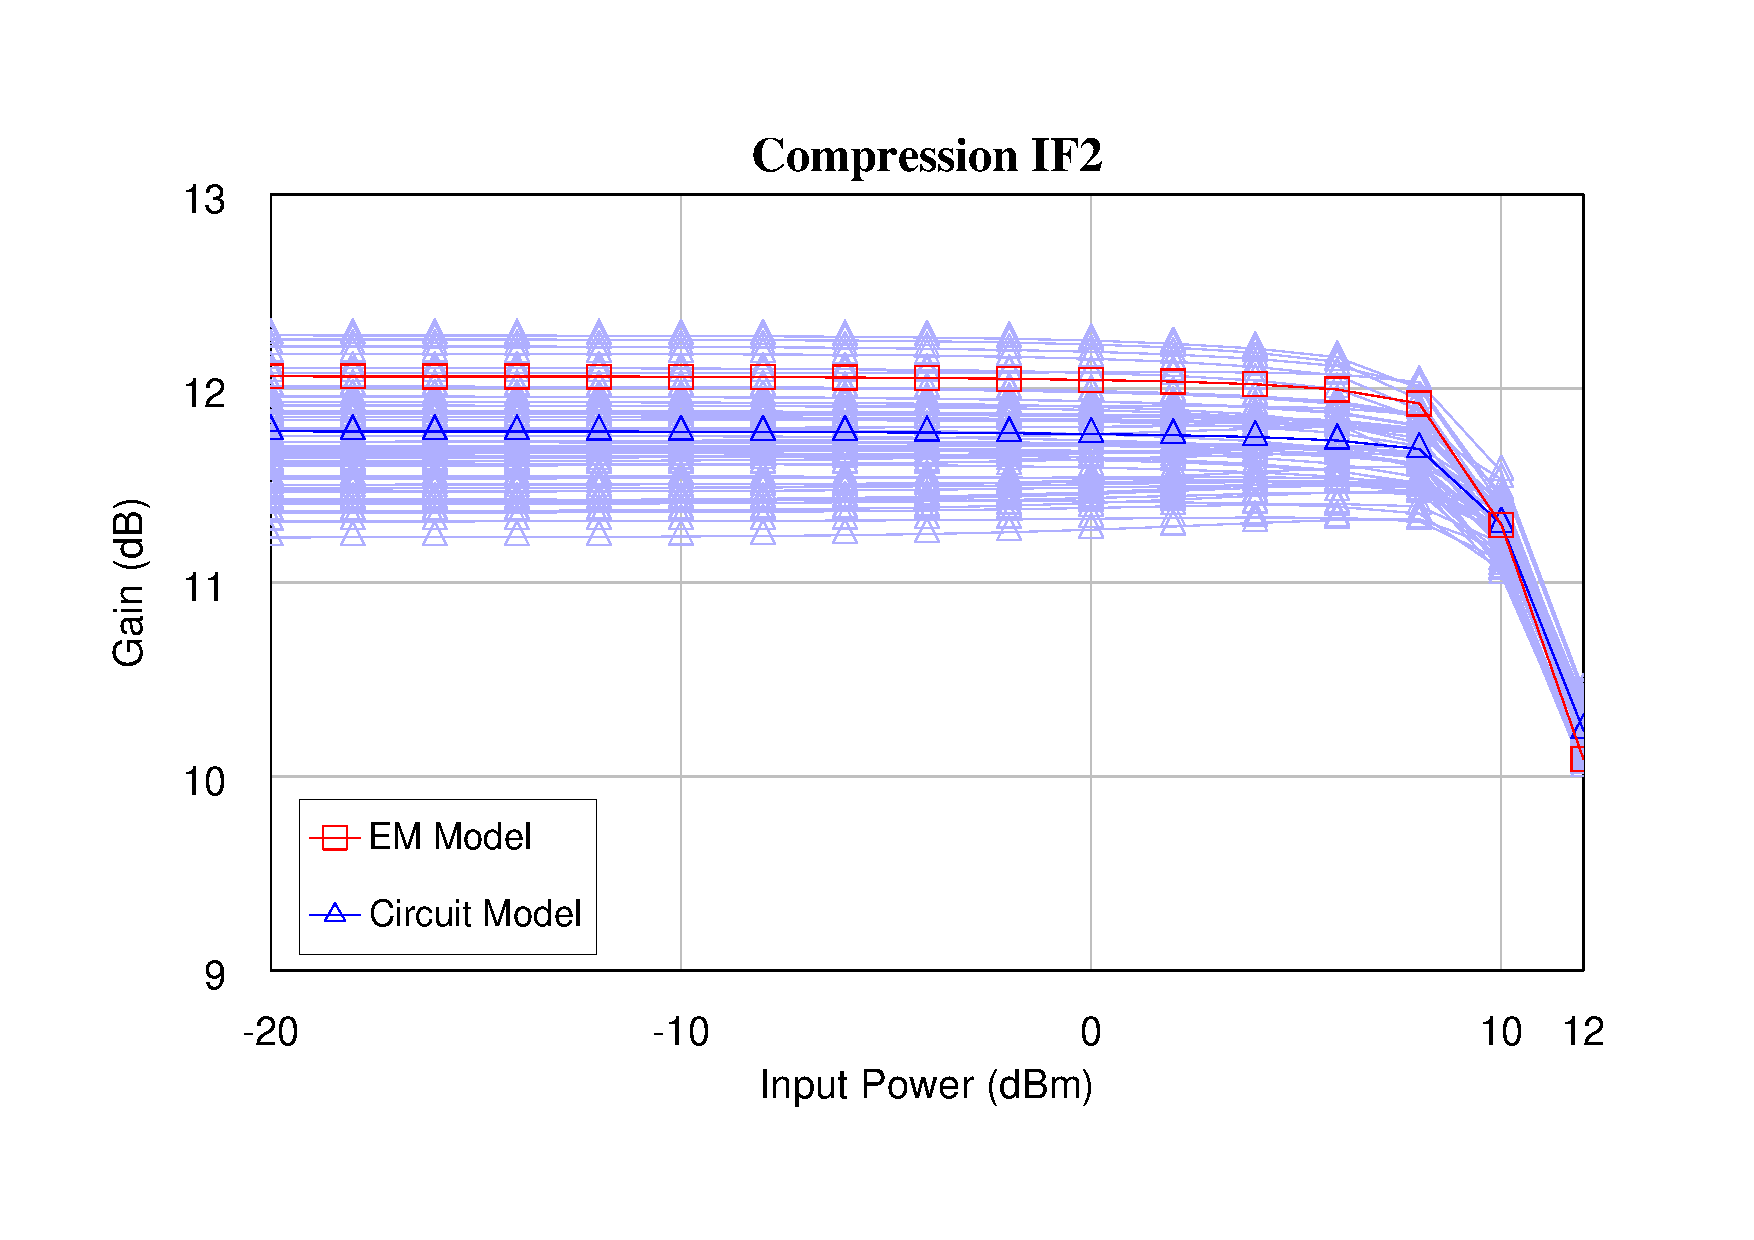
\includegraphics[width=0.9\textwidth]{fig/yield/compressif2}
%			\includerect{1.0\textwidth}{fig/yield/compressif2}
%			\caption[Yield analysis of the power compression for amplifier IF2.]{Power compression of amplifier IF 2 \unit[2.14]{GHz}. The spread analyzed with the electric circuit model gives a hint of the spread for the more accurate electromagnetic simulation.}\label{fig:yieldif2compress}
%		\end{figure}
%		
%		\begin{figure}[hbt!]
%			\centering
%			%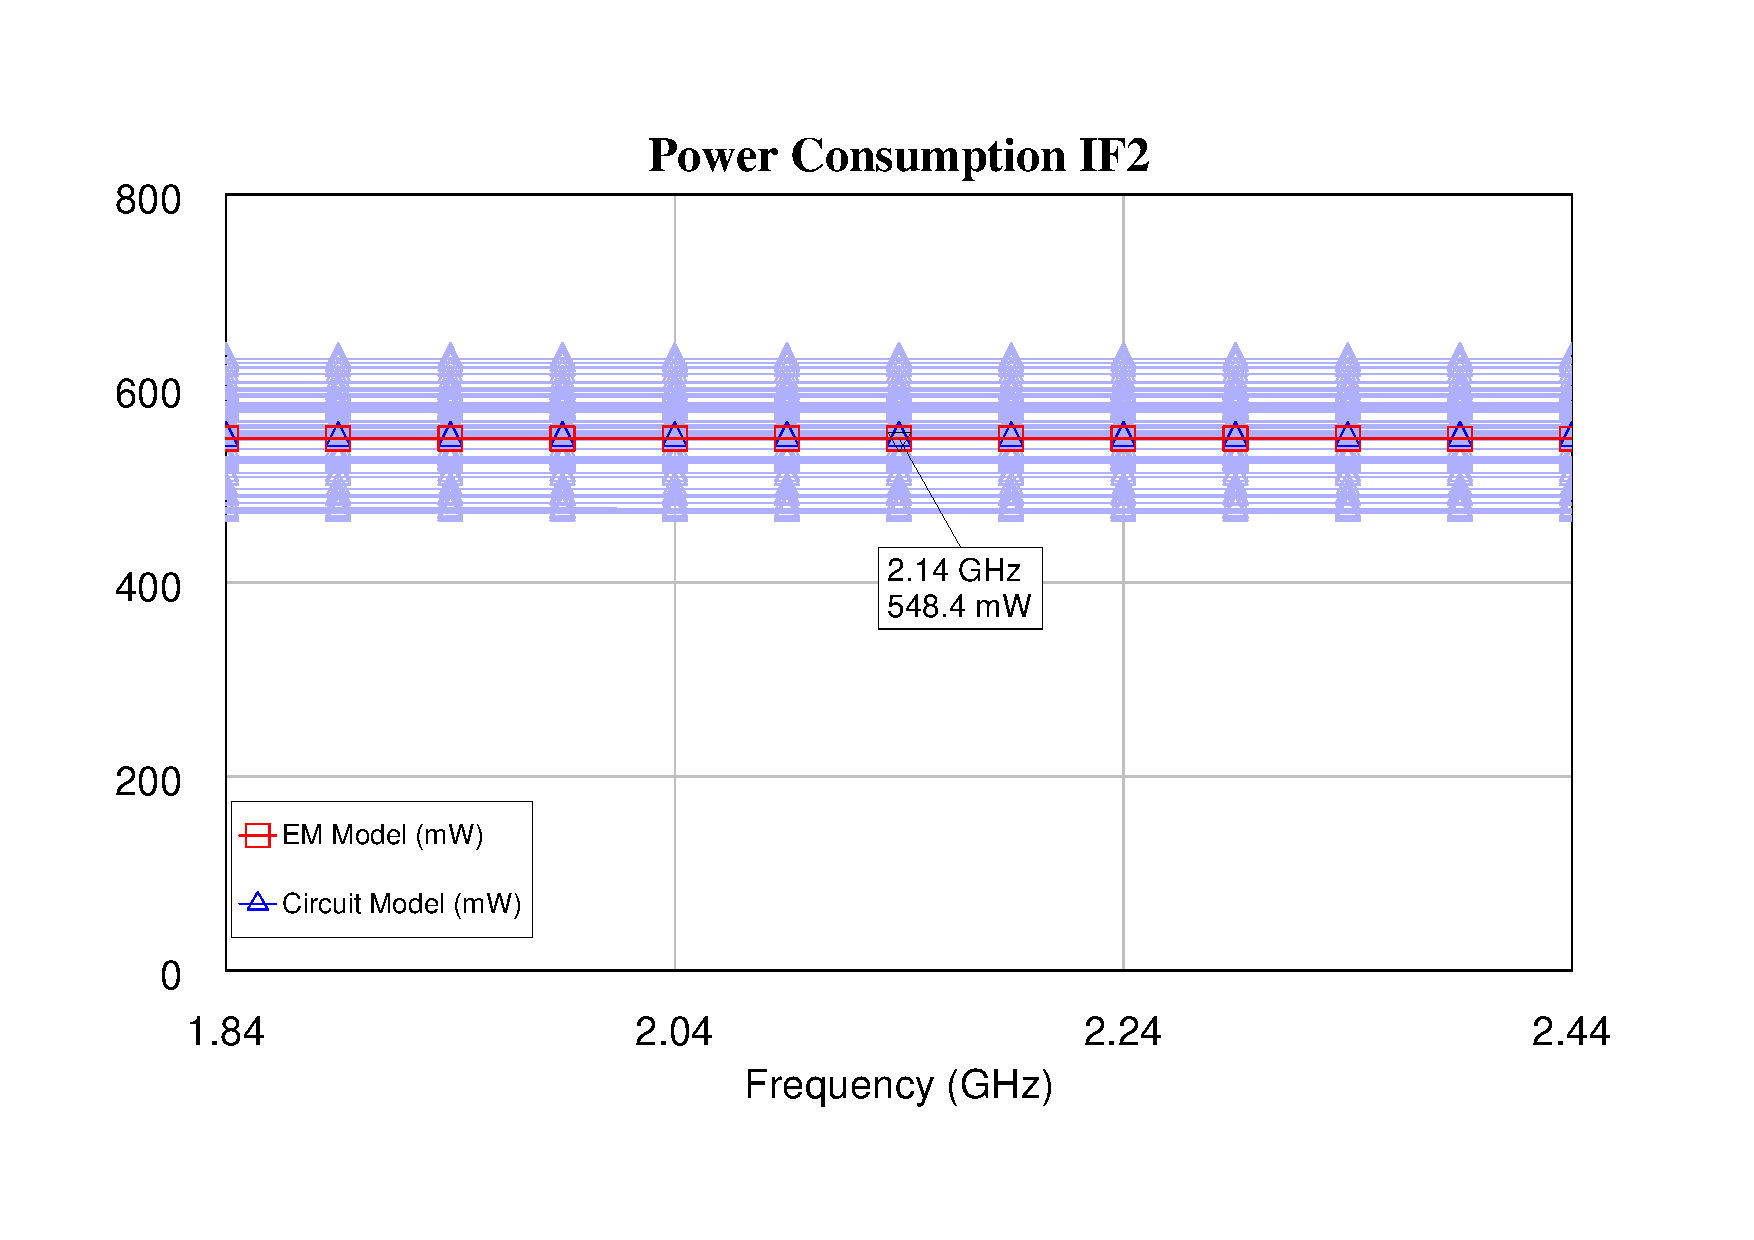
\includegraphics[width=0.9\textwidth]{fig/yield/powerif2}
%			\includerect{1.0\textwidth}{fig/yield/powerif2}
%			\caption[Yield analysis of power consumption for amplifier IF2.]{Power consumption of amplifier IF 2. The spread analysed with the electric circuit model gives a hint of the spread for the more accurate electromagnetic simulation.}\label{fig:yieldif2power}
%		\end{figure}


	\section{Mixer}
		Yield analysis of the mixer's input matching and conversion gain as well as the stand-alone diplexer are shown in \autoref{fig:yieldmixer}. All yield results are concluded in \autoref{tab:yieldmixer}.
		
		\begin{table}[hbt!]
			\caption[Mixer performance with spread.]{Typical mixer performance with spread at input power \unit[-2]{dBm}.}
			\label{tab:yieldmixer}
			\centering
			\begin{tabular}{ l l l l } \toprule
				Parameter & Performance & Performance & Unit \\\midrule
				Band & 2.9--3.4 & 3.1--3.3 & GHz \\\midrule
				Conversion loss & $7.7\pm 0.8$ & $7.5\pm 0.8$ & dB \\
				Gain variation & $0.45\pm 0.4$ & $0.05\pm 0.3$ & dB \\
				Return loss input & $16\pm 3$ & $21\pm 5$ & dB \\
				Return loss output (@\unit[2.14]{GHz}) & $16\pm 2$ & $16\pm 2$ & dB \\
				$P_{1dB}$ (input) & $13\pm 0$ & $13\pm 0.5$ & dBm \\\bottomrule
			\end{tabular}
		\end{table}
		
		\begin{figure}[hbt!]
			\centering 
			\subfloat[][]{
				\includerect{0.5\textwidth}{fig/yield/mixermatchyield}
				\label{fig:yieldmatch}
			}
			\subfloat[][]{
				\includerect{0.5\textwidth}{fig/yield/convgainyield}
				\label{fig:yieldconvgain}
			}\\
			\subfloat[][Yield analysis of the diplexer. The red (single) lines are the EM simulations and the blue (broad) lines correspond to the spread analysed with the circuit model. The curves marked with triangles $\triangle$ details the bandpass filter between the RF input and the mixer-FET's drain. The curves marked with squares $\medsquare$ details the low-pass filter between the mixer-FET's drain and the IF output.]{
				\includerect{1.0\textwidth}{fig/yield/diplexer}
				\label{fig:yielddiplexer}
			}
			\caption[Mixer yield analysis.]{Yield analysis of \subref{fig:yieldmatch} the RF input matching \subref{fig:yieldconvgain} the mixer's conversion gain and \subref{fig:yielddiplexer} the diplexer. The spread analysed with the electric circuit model gives a hint of the spread for the more accurate electromagnetic simulation.}\label{fig:yieldmixer}
		\end{figure}
		
		
	\section{Chip}
		Yield analysis of chip conversion gain is shown in \autoref{fig:yield_chip_gain}. 
		
			\begin{figure}[hbt!]
				\centering
				\includerect{0.7\textwidth}{fig/yield/chip_gain_spread_T55}
				\caption[Spread on chip conversion gain.]{Yield analysis on chip conversion gain at \unit[55]{$^\circ$C} and nominal gain. Circuit models are used. The yield is \unit[$\pm1$]{dB}. Other temperatures show similar spread.}\label{fig:yield_chip_gain}
			\end{figure}